\section{Method}

\label{sec:method}

The method diagram contrasts the two executed paths from a shared fact episode to a fresh query conversation and a paired audit. The baseline constructs a file-derived section and retains its prefix. The retrieved arm constructs dialogue-shaped memory items, ranks them, and packs complete formatted items into the allowed section. The same model answers both queries, but construction and presentation differ jointly. Accordingly, the estimand is the observed difference between these operational systems under a matched section budget, rather than the isolated effect of lexical retrieval.


\begin{figure}[htbp]
\centering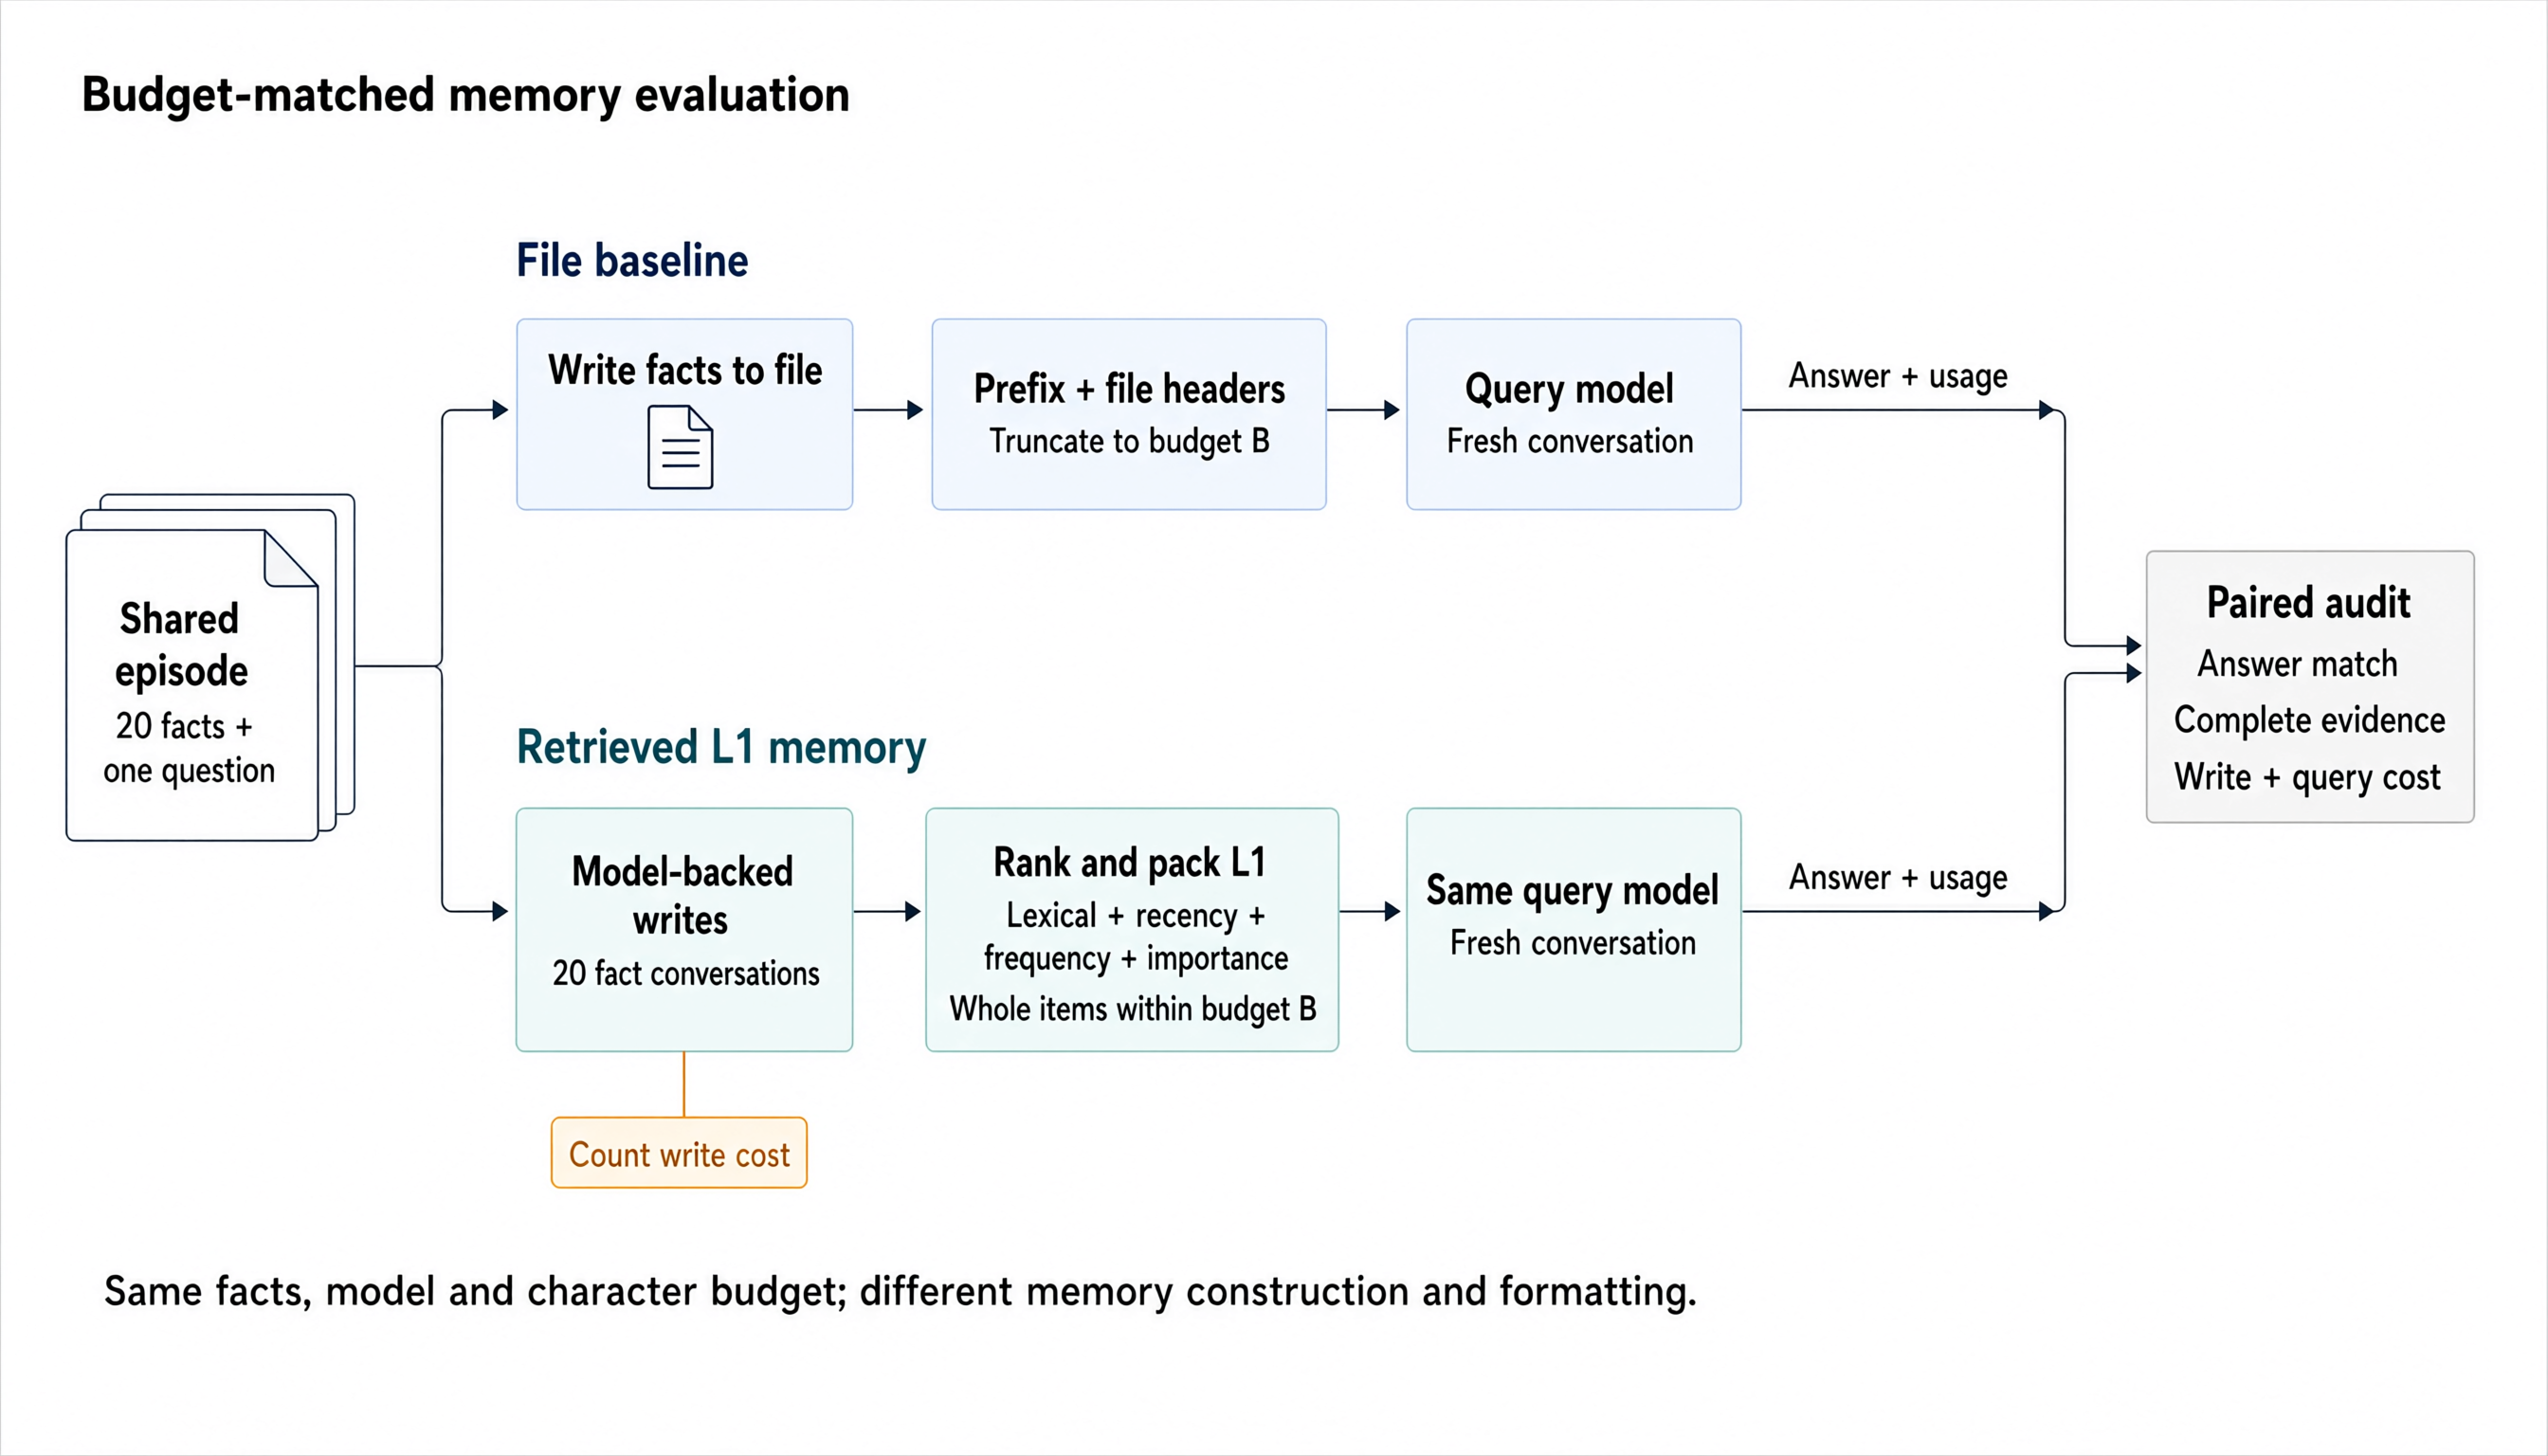
\includegraphics[width=\linewidth]{figures/methodology.png}
\caption{Budget-matched evaluation of two operational memory paths. The retrieved arm
incurs model-backed write cost before its isolated query. Equal character caps include
each arm's own formatting overhead. This schematic illustrates the audited implementation;
it is not an experimental result.}
\label{fig:methodology}\end{figure}
\subsection{Frozen Memory and Matched Token Packing}

\label{sec:method_baseline}

The baseline uses ProjectMemoryRail. Facts are written directly to an isolated JIUWENSWARM.md file without model-backed seeding. At query time, the runner reads the file, includes its filename and modification metadata, and truncates the complete memory section to the allowed prefix. All of these characters count against the budget. There is no query-dependent reordering: later facts can be removed regardless of relevance, and the truncation boundary may split a fact. Consequently, the arm is a concrete file-prefix baseline rather than an embedding retriever. If complete evidence is absent, that establishes what the model did not receive under this protocol; it does not establish how a differently ordered or reformatted file would perform.

\subsection{Contrastive Tier-Based Lexical Selection (CTLS)}

\label{sec:method_ctls}

CTLS (Contrastive Tier-Based Lexical Selection) is a novel selector that partitions the candidate set into a lexically relevant tier (Jaccard overlap J(q,m) greater than zero) and a lexically absent tier (J(q,m) equal to zero) before applying any temporal scoring. Within the relevant tier, candidates are ranked by the full hybrid score, so temporal decay and frequency serve as tiebreakers among genuinely relevant items. Within the absent tier, recency plus importance ranks candidates for fallback. Packing draws from the relevant tier first, then from the absent tier if budget permits. This partition provably satisfies a Non-Dominance Property: for any candidate with positive overlap and any candidate with zero overlap, CTLS always ranks the positive-overlap item first, regardless of freshness gap. The mechanism inequality (Equation dom\_condition) shows precisely why the original hybrid fails: a fixed query-independent freshness weight can outweigh a positive lexical advantage, displacing a relevant older record with a fresher but irrelevant one. The tier partition eliminates this by construction. \citep{ref_959d6858d034c6e1}

CTLS requires no model calls, no learned parameters, and no embedding model beyond the existing lexical tokenizer already in the pipeline. It is a zero-cost selector substitution over the frozen candidate bank. The implementation uses the same whole-item greedy packer as the baseline hybrid, differing only in candidate ordering. The hybrid\_no\_time ablation (temporal weight set to zero globally) is the theoretical limit case of CTLS when every candidate has positive overlap; their empirical gap on each budget measures the value of within-tier temporal tiebreaking rather than eliminating it. \citep{ref_ab2c226739f2f52a}

\subsection{Repeated Real Agent Evaluation and Ablation Design}

\label{sec:method_protocol}

Each memory episode has its own fact set and fresh agent instances. The frozen bank design holds source records, timestamps, metadata, and segment content fixed across all selectors; write tokens are zero and construction cost is identical across every arm. The formal question uses a new conversation ID so that no seeding dialogue leaks into the query context. The runner verifies isolated query history and confirms actual memory injection before scoring. \citep{ref_ab2c226739f2f52a}

Evidence recall requires the complete annotated turn to appear in the delivered context; evidence-session recall requires any segment from the annotated session to be selected. Three answering calls per memory episode are averaged before stratified cluster bootstrap inference with Holm correction across all prespecified comparisons. The evaluation design adapts the stratified extraction paradigm of LongMemEval; the resulting subset is not an official benchmark score.

\FloatBarrier

\subsection{Budget and cost formalization}
Let $q$ be a question, $M$ its episode memory, and $B$ the cap on the entire
injected memory section, including headings and metadata. The baseline constructs
a file-derived section and keeps its prefix. The retrieved arm scores stored
exchanges, takes at most $k=10$ candidates, and greedily appends complete formatted
items that fit. An over-budget item is skipped rather than partially appended;
later smaller items can still be considered. Thus equal $B$ does not imply equal
usable fact content or identical prompt formatting.
\begin{equation}
  s(q,m)=0.4J(T(q),T(m))+0.3\,2^{-a(m)/h}
       +0.2\min\!\left\{\frac{\log(1+f(m))}{\log(101)},1\right\}+0.1I(m),
  \label{eq:ranking}
\end{equation}
where $T$ lowercases text and keeps alphanumeric/underscore word tokens longer
than one character; $J(A,C)=|A\cap C|/|A\cup C|$ (zero for an empty set);
$a(m)$ is age in seconds; $h=86400$ is the decay half-life; $f(m)$ is the recorded
access count; and $I(m)$ is a bounded heuristic importance score. These are the
implementation's default weights, not learned or tuned coefficients. No embedding
model is invoked. L1 holds at most 20 exchanges with a one-hour time-to-live;
individual displayed exchanges are capped at 500 characters before packing.

The cost estimand includes initialization through model-backed memory writes:
\begin{equation}
 C_g=\frac{\sum_{r\in\mathcal{Q}_g}u_r+
                 \sum_{w\in\mathcal{W}_g}u_w}{N_{\rm valid}},\qquad
 L_g=\frac{\sum_{r\in\mathcal{Q}_g}t_r+
                 \sum_{w\in\mathcal{W}_g}t_w}{N_{\rm valid}}.
 \label{eq:accounting}
\end{equation}
Here $u$ and $t$ denote recorded token usage and elapsed time, respectively;
$\mathcal Q_g$ and $\mathcal W_g$ include all recorded query and write attempts.
The denominator counts valid matched question pairs. These timing sums exclude
unrecorded process initialization and are not a full application wall-clock time.
Missing usage remains unknown rather than zero.

For each valid pair, let $y_{g,i}$ indicate an accepted-answer substring match
and $e_{g,i}$ indicate that the complete target fact survived in the injected text:
\begin{equation}
 A_g=\frac{1}{N}\sum_i y_{g,i},\qquad
 R_g=\frac{1}{N}\sum_i e_{g,i},\qquad
 \Delta A=A_{\rm retrieved}-A_{\rm file}.
 \label{eq:metrics}
\end{equation}
The two indicators differ: a truncated fact can contain a sufficient answer span.
Wilson intervals describe finite-question uncertainty only. They do not estimate
model-run variability, correct the selected slice's bias, or establish significance.

\begin{table}[htbp]
\centering\small
\caption{Audited execution protocol. No component ablation or weight tuning is claimed.}
\label{tab:protocol}
\begin{tabular}{p{0.25\linewidth}p{0.66\linewidth}}\toprule
Step & Operation \\\midrule
Prepare & Create fresh isolated agents; give both arms the same fact episode. \\
Construct & Write the baseline file; seed retrieved L1 through separate fact conversations. \\
Query & Use a fresh conversation, no tools, one model iteration, and the assigned section budget. \\
Audit & Check actual prompt injection and isolated history before accepting a pair. \\
Aggregate & Match question IDs; count writes once per run; preserve excluded attempts in costs. \\
\bottomrule\end{tabular}\end{table}

\FloatBarrier
